% !TEX root = saveliev_physics_general_course_2.tex
%!TEX TS-program = pdflatex
%!TEX encoding = UTF-8 Unicode


\chapter[DÒNG ĐIỆN TRONG CHẤT KHÍ]{DÒNG ĐIỆN TRONG CHẤT KHÍ}\label{chap:12}

\chaptermark{DÒNG ĐIỆN 
TRONG CHẤT KHÍ}

\section{Dẫn điện bán duy trì và tự duy trì}\label{sec:12_1}

Sự dẫn điện qua một chất khí được gọi là \textbf{phóng điện}.
Các chất khí tại trạng thái thông thường đều cách điện và không tồn tại các hạt tải điện.
Chỉ khi có các điều kiện đặc biệt thì các hạt tải (ion, electron) mới tồn tại và sự phóng điện diễn ra.

Các hạt tải điện có thể tồn tại trong chất khí do các tác nhân bên ngoài không liên quan đến sự tồn tại của điện trường.
Trong trường hợp này, chất khí đang có \textbf{dẫn điện bán duy trì}
Sự phóng điện bán duy trì có thể diễn ra do sự đun nóng một chất khí (ion hóa nhiệt), tác động của các tia cực tím hoặc tia X, và cũng có thể do phóng xạ.

Nếu các hạt tải điện xuất hiện do tác dụng của điện trường bên trong chất khí, sự dẫn điện được gọi là \textbf{tự duy trì}.
Bản chất của sự phóng điện phụ thuộc vào nhiều yếu tố: vào tính chất hóa học của chất khí và các điện cực, vào nhiệt độ và áp suất của chất khí, vào hình dạng, kích thước và cách bố trí 
của các điện cực, vào điện áp đặt lên điện cực, vào mật độ và cường độ dòng điện, v.v.
Đây chính là lý do sự phóng điện trong chất khí có thể có nhiều dạng rất khác nhau.
Một vài kiểu phóng điện có đi kèm với hiệu ứng âm thanh và ánh sáng---chẳng hạn như sấm chớp.

\section{Phóng điện bán duy trì}\label{sec:12_2}

Cho một chất khí với hai điện cực (\fig{12_1}) chịu tác dụng của một tác nhân ion hóa (chẳng hạn như tia X).
Sự ion hóa này khiến một hoặc nhiều electron bị tách rời khỏi các phân tử khí.
Các phân tử khí này sau đó trở thành các ion tích điện dương.
Tại áp suất không quá thấp, phần lớn các electron sẽ bị các phân tử trung hòa về điện giữ lại và trở thành các ion tích điện âm.
Đặt $\Delta{\ab{n}{i}}$ ký hiệu cho số cặp ion xuất hiện do tác động của sự ion hóa trong một đơn vị thể tích trên một giây.

\begin{figure}[t]
	\begin{center}
		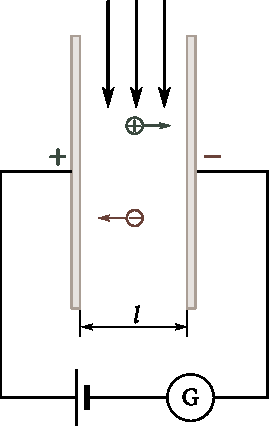
\includegraphics[scale=1]{figures/ch_12/fig_12_1.pdf}
		\caption[]{}
		\label{fig:12_1}
	\end{center}
	\vspace{-0.8cm}
\end{figure}

Quá trình ion hóa một chất khí diễn ra kèm theo sự tái hợp của các ion, \ie, sự trung hòa điện tích của các ion trái dấu khi chúng va vào nhau hoặc sự tạo thành một phân tử trung hòa bởi một ion dương và một electron.

Khả năng hai ion trái dấu va vào nhau tỉ lệ thuận với số lượng của cả các ion dương và ion âm.
Do đó, số cặp ion $\Delta{\ab{n}{r}}$ tái hợp trong một đơn vị thể tích trên một giây tỉ lệ thuận với bình phương số cặp ion $n$ trong một đơn vị thể tích:
\begin{equation}\label{eq:12_1}
    \Delta{\ab{n}{r}} = rn^2
\end{equation}

\noindent
($r$ là hằng số tỉ lệ).

Tại trạng thái cân bằng, số lượng ion xuất hiện bằng số lượng ion tái hợp, do đó
\begin{equation}\label{eq:12_2}
    \Delta{\ab{n}{i}} = rn^2.
\end{equation}

\noindent
Ta có biểu thức sau cho mật độ ion cân bằng (số cặp ion trong một đơn vị thể tích)
\begin{equation}\label{eq:12_3}
    n = \parenthesis{\frac{\Delta{\ab{n}{i}}}{r}}^{1/2}.
\end{equation}

Khoảng vài cặp ion xuất hiện mỗi giây trong một \SI{1}{\centi\metre} quyển dưới tác động của bức xạ vũ trụ và các chất phóng xạ trong vỏ Trái đất.
Giá trị hằng số $r$ cho không khí là \SI{1.6e-6}{\centi\metre\cubed\per\second}.
Thay các giá trị này vào \eqn{12_3} cho kết quả mật độ ion cân bằng trong không khí vào khoảng \SI{e3}{\centi\metre\cubed}
Mật độ này không đủ lớn để sự dẫn điện có thể được chú ý đến.
Không khí khô tinh khiết là vật cách điện rất tốt.

Nếu chúng ta đặt điện áp vào các điện cực, số ion sẽ giảm đi, không chỉ vì sự tái hợp, mà còn do các ion bị kéo lại do điện trường từ các điện cực.
Giả sử như $\Delta{\ab{n}{j}}$ cặp ion bị kéo lại từ mỗi đơn vị thể tích trong một giây.
Nếu điện tích mỗi ion là $e'$, khi đó sự trung hòa của một cặp điện tích trên các điện cực tương ứng với một điện tích $e'$ di chuyển dọc theo mạch
Cứ mỗi giây, $\Delta{\ab{n}{j}}Sl$ cặp ion bị giữ lại bởi các điện cực (ở đây $S$ là tiết diện các điện cưc, $l$ là khoảng cách giữa chúng và tích $Sl$ bằng thể tích không gian giữa các điện cực).
Do đó, dòng điện trong mạch là
\begin{equation*}
    I = e' \Delta{\ab{n}{j}} Sl,
\end{equation*}

\noindent
với
\begin{equation}\label{eq:12_4}
    \Delta{\ab{n}{j}} = \frac{I}{e' l S} = \frac{j}{e' l},
\end{equation}

\noindent
với $j$ là mật độ dòng điện.

Khi có dòng điện chạy qua, tồn tại điều kiện cân bằng sau:
\begin{equation*}
    \Delta{\ab{n}{i}} = \Delta{\ab{n}{r}} + \Delta{\ab{n}{j}}
\end{equation*}

\noindent
Thế vào $\Delta{\ab{n}{r}}$ và $\Delta{\ab{n}{j}}$ giá trị của chúng từ \eqns{12_1}{12_4}, ta có phương trình
\begin{equation}\label{eq:12_5}
    \Delta{\ab{n}{i}} = rn^2 + \frac{j}{e' l}.
\end{equation}

Mật độ dòng được xác định bởi biểu thức
\begin{equation}\label{eq:12_6}
    j = e' n \parenthesis{u_0^+ + u_0^-} E,
\end{equation}

\noindent
với $u_0^+$ và $u_0^-$ lần lượt là hoạt tính của các ion dương và âm [tham khảo \eqn{11_17}].

Hãy khảo sát hai trường hợp giới hạn---trường yếu và mạnh.

Với các trường yếu, mật độ dòng sẽ rất nhỏ, và số hạng $j/(e'l)$ trong \eqn{12_5} có thể bỏ qua khi so với $rn^2$ (điều này thể hiện rằng ion rời không gian giữa các điện cực chủ yếu do sự tái hợp)
Phương trình \eqref{eq:12_5} trở thành \eqn{12_2}, và ta nhận được \eqn{12_3} cho mật độ ion cân bằng.
Từ giá trị của $n$ tại \eqn{12_6}, ta có
\begin{equation}\label{eq:12_7}
    j = e' \parenthesis{\frac{\Delta{\ab{n}{i}}}{r}}^{1/2} \parenthesis{u_0^+ + u_0^-} E.
\end{equation}

\noindent
Nhân tử trước $E$ trong \eqn{12_7} không phụ thuộc vào cường độ trường.
Do đó, với giá trị của trường yếu, sự phóng điện bán duy trì tuân thủ định luật Ohm.

Hoạt tính của các ion trong chất khi có cỡ giá trị khoảng \SI{e-4}{\metre\squared\per\volt\per\second} [or \SI{1}{\centi\metre\squared\per\volt\per\second}]. Do đó, tại trạng thái cân bằng  $n = \SI{e3}{\per\centi\metre\cubed} = \SI{e9}{\per\metre\cubed}$ và cường độ trường $E = \SI{1}{\volt\per\metre}$, mật độ dòng sẽ bằng
\begin{equation*}
    j = \num{1.6e-19} \times \num{e9} \parenthesis{\num{e-4}+\num{e-4}} \times 1 \sim \SI{e-14}{\ampere\per\metre\squared} = \SI{e-18}{\ampere\per\centi\metre\squared}
\end{equation*}

\noindent
[tham khảo \eqn{12_6}; giả thiết các ion tích điện nhẹ].

Với giả thiết trường mạnh, ta có thể bỏ qua số hạng $rn^2$ trong \eqn{12_5} so với $j/e'l$.
Điều này thể hiện rằng gần như tất cả các ion xuất hiện sẽ va vào điện cực trước khi có thời gian để tái hợp.
Trong những điều kiện này, \eqn{12_5} trở thành
\begin{equation*}
    \Delta{\ab{n}{i}} = \frac{j}{e' l},
\end{equation*}

\noindent
với
\begin{equation}\label{eq:12_8}
    j = e' \Delta{\ab{n}{i}} l.
\end{equation}

\noindent
Mật độ dòng này được sinh ra bởi tất cả các ion xuất phát từ các điểm ion hóa trong một cột khí nằm giữa các điện cực.
Do đó, mật độ dòng này lớn nhất tại giá trị cho trước của ion hóa [?] và khoảng cách $l$ giữa các điện cực.
Giá trị này được gọi là mật độ dòng bão hòa $\ab{j}{sat}$

Ta hãy tính $\ab{j}{sat}$ với các điều kiện sau: $\Delta{\ab{n}{i}} = \SI{e-3}{\per\centi\metre\cubed}$ (đây xấp xỉ mật độ hình thành ion tại không khí ở các điều kiện thường), $l = \SI{0.1}{\metre}$.
Đưa những dữ liệu này vào \eqn{12_8} cho ta
\begin{equation*}
    \ab{j}{sat} = \num{1.6e-19} \times \num{e7} \times \num{e1} \sim \SI{e-13}{\ampere\per\metre\squared} = \SI{e-17}{\ampere\per\centi\metre\squared}.
\end{equation*}

\noindent
Những kết quả này cho thấy rằng sự dẫn điện của không khí trong điều kiện thường là không đáng kể.

\begin{figure}[t]
	\begin{center}
		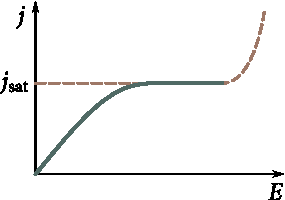
\includegraphics[scale=1]{figures/ch_12/fig_12_2.pdf}
		\caption[]{}
		\label{fig:12_2}
	\end{center}
	\vspace{-0.8cm}
\end{figure}

Tại các giá trị trung gian của $E$, có sự chuyển tiếp mượt từ pha phụ thuộc tuyến tính của $j$ vào $E$ cho tới khi bão hòa; khi sự bão hòa diễn ra, $j$ ngừng phụ thuộc vào $E$ (tham khảo đường cong tại $\fig{12_2}$.
Vùng bão hòa được tiếp nối bởi vùng có sự tăng mạnh của dòng điện (hãy quan sát phần đường cong được vẽ bằng nét đứt).
Lý giải cho điều này là bắt đầu từ một giá trị nhất định của $E$, các electron\footnote{Do quãng đường tự do trung bình của chúng lớn hơn, các electron nhận được khả năng ion hóa do va chạm sớm hơn của các ion khí} sinh ra bởi các nguồn ion hóa ngoài nhận được năng lượng đáng kể khi đang trên quỹ đạo tự do.
Năng lượng này đủ để ion hóa các phân tử chúng va chạm.
Các ion tự do sản sinh ra trong sự ion hóa này, sau khi tăng tốc, tiếp tục gây ra sự ion hóa.
Từ đó, sự sản sinh dây chuyền các ion chính do tác nhân ion hóa bên ngoài diễn ra, và dòng phóng điện được nhân lên nhiều lần
Quá trình này không mất đi bản chất của một sự phóng điện 
bán duy trì, do sau khi tác nhân ion hóa ngoài dừng lại, sự phóng điện chỉ tiếp tục đến khi tất cả các electron (chính và thứ cấp) đến được anode (biên của không gian chứa các hạt ion hóa---electron---di chuyển về phía anode).
Để một sự phóng điện tự duy trì, cần có hai dòng ion phản ứng dây chuyền va vào nhau/
Điều này chỉ diễn ra khi sự ion hóa do va chạm có khả năng sinh ra các hạt tải điện mang điện trái dấu.

Ta cần chú ý rằng các dòng phóng điện bán duy trì được nhân lên bởi sự sinh ra của các hạt tải điện tỉ lệ thuận với số các ion chính được sinh ra bởi tác nhân ion hóa ngoài.
Tính chất này của sự phóng điện được dùng trong các bộ đếm tỉ lệ (tham khảo các phần sau).

\section{Buồng Ion và bộ đếm}\label{sec:12_3}

Các buồng ion hóa và máy đếm được sử dụng để phát hiện và đếm các hạt cơ bản, cũng như đo đạc cường độ của các tia X và tia gamma.
Khả năng của các dụng cụ trên được dựa vào sự phóng điện bán duy trì trong chất khí.

\begin{figure}[t]
	\begin{center}
		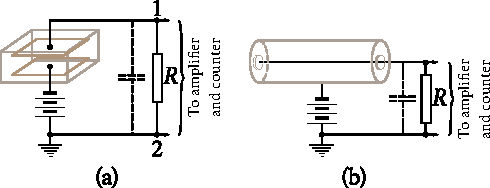
\includegraphics[scale=1]{figures/ch_12/fig_12_3.pdf}
		\caption[]{}
		\label{fig:12_3}
	\end{center}
	\vspace{-0.8cm}
\end{figure}

Sơ đồ của một buồng ion hóa và một bộ đếm là như nhau (\fig{12_3}).
Chúng chỉ khác nhau về điều kiện hoạt động và các tính năng cấu trúc.
Một bộ đếm (\fig{12_3}b) bao gồm một thân máy hình trụ có một dây mỏng (anode) được duỗi ra gắn vào các trụ cách điện.
Thân máy của bộ đếm chính là cathode.
Một màn mica hoặc nhôm được đặt tại một đầu của máy đếm để nhận các hạt ion hóa.
Một số hạt, cũng như tia X và tia gamma có thể xuyên vào máy đếm hoặc buồng ion hóa trực tiếp qua lớp tường của chúng.
Một buồng ion hóa (\fig{12_3}b) có các điện cực với nhiều hình dạng khác nhau.
Cụ thể hơn, chúng có thể giống như một bộ đếm nhưng có hình dạng của các tấm phẳng, ...

Giả thiết rằng một hạt tích điện tốc độ cao sinh ra $N_0$ cặp các ion chính (electron và các ion dương) bay vào không gian giữa các điện cực.
Các ion này được điện trường đưa vào không gian giữa các điện cực, và do đó, một điện tích nhất định $q$ mà chúng ta sẽ gọi là một xung dòng điện, chạy qua điện trở $R$.
Hình \ref{fig:12_4} cho thấy liên hệ giữa xung dòng $q$ và điện áp $U$ giữa các điện cực với hai lượng ion chính $N_0$ khác nhau ba lần ($N_{02} = 3N_{01}$.
Đồ thị này có thể được chia thành sáu vùng.
Vùng I và II đã được khảo sát ở phần trước.
Cụ thể hơn, vùng II là khu vực của dòng điện bão hòa---tất các các ion sinh ra bởi hạt ion hóa đến được các điện cực mà không có 
thời gian để tái hợp.
Dĩ nhiên, trong điều kiện này xung dòng điện không phụ thuộc vào điện áp.

Kể từ giá trị $\ab{U}{p}$, cường độ điện trường đủ lớn để các electron có khả năng ion hóa các phân tử bằng va chạm. Do đó, lượng electron và ion dương tăng đột ngột như một phản ứng dây chuyền.
Theo đó, $AN_0$ ion chạm đến các điện cực.
Đại lượng $A$ được gọi là \textbf{hệ số khuếch đại chất khí}.
Tại vùng III, hệ số này không phụ thuộc vào số ion chính (nhưng có phụ thuộc vào điện áp).
Do đó, nếu ta giữ nguyên điện áp, xung dòng điện sẽ tỉ lệ thuận với số ion chính.
Vùng III được gọi là \textbf{vùng tuyến tính}, và điện áp $\ab{U}{p}$ gọi là \textbf{ngưỡng của vùng tuyến tính}.
Hệ số khuếch đại chất khí thay đổi trong vùng này từ $1$ tại điểm đầu đến \num{e3}-\num{e4} tại điểm cuối (\fig{12_4} chưa có tỉ lệ xích theo trục $q$; chỉ có tỉ lệ $1$:$3$ giữa tọa độ trong 
vùng II và III).

\begin{figure}[t]
	\begin{center}
		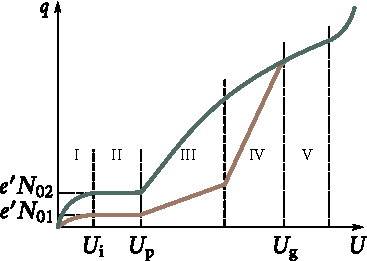
\includegraphics[scale=1]{figures/ch_12/fig_12_4.pdf}
		\caption[]{}
		\label{fig:12_4}
	\end{center}
	\vspace{-0.8cm}
\end{figure}

Tại vùng IV, được gọi là \textbf{vùng tuyến tính từng phần}, hệ số khuếch đại $A$ phụ thuộc ngày càng nhiều vào $N_0$.
Tại vùng này, chênh lệch giữa xung dòng điện sinh ra bởi các giá trị khác nhau của số ion chính trở nên càng ít dần đi.

Tại điện áp tương ứng với vùng V(còn được biết là \textbf{vùng Geiger}, và điện áp $\ab{U}{g}$ là ngưỡng của vùng này), quá trình này bắt đầu có những tính chất của sự phóng điện bán duy trì.
Các ion chính sinh ra càng kéo theo sự xuất hiện của nhiều ion thêm nữa.
Xung dòng điện ở vùng này hoàn toàn không phụ thuộc vào số lượng ion chính

Tại vùng VI, điện áp cao đến mức sự phóng điện, sau khi được bắt đầu, sẽ không dừng lại.
Do đó, nó được gọi là \textbf{vùng phóng điện liên tục}.

\textbf{Buồng Ion hóa}. Một buồng ion hóa là một dụng cụ hoạt động không dựa vào sự khuếch đại chất khí, \ie, tại điện áp tương ứng với vùng II.
Có hai loại buồng ion hóa.
Một loại buồng được dùng để ghi nhận các xung tín hiệu xuất phát từ các hạt đơn lẻ (buồng xung).
Một hạt bay qua buồng sinh ra một lượng ion nhất định, và do đó dòng điện $I$ bắt đầu chạy qua điện trở $R$.
Kết quả là điện áp của điểm $1$ (\fig{12_3}a) tăng lên và bằng $IR$ (điện áp ban đầu của điểm này bằng với điểm nối đất $2$).
Điện áp này được đưa đến một mạch khuếch đại, và sau khi được khuếch đại, tín hiệu được đưa vào bộ đếm.
Sau khi tát cả các điện tích đến được điện cực phía trong đi qua điện trở $R$, dòng điện ngưng lại và điện áp của điểm $1$ lại một lần nữa bằng 0.
Bản chất của buồng này phụ thuộc vào khoảng thời gian của xung dòng điện gây ra bởi một hạt ion hóa.

\begin{figure}[t]
	\begin{center}
		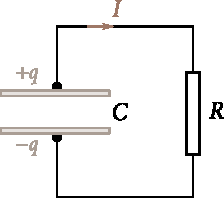
\includegraphics[scale=1]{figures/ch_12/fig_12_5.pdf}
		\caption[]{}
		\label{fig:12_5}
	\end{center}
	\vspace{-0.8cm}
\end{figure}

Để xác định thời gian của một xung, hãy xét mạch điện gồm tụ $C$ và trở $R$ (\fig{12_5}).
Nếu ta nạp các điện tích $+q$ và $-q$ vào các bản tụ, dòng điện sẽ chạy qua điện trở $R$ và các điện tích trên bản sẽ giảm dần.
Điện áp tức thời trên điện trở là $U = q/C$.
Từ đó ta có biểu thức cho dòng điện.
\begin{equation}\label{eq:12_9}
    I = \frac{U}{R} = \frac{q}{RC}.
\end{equation}

\noindent
Ta thế $-\diffin{q}{t}$ cho dòng điện, với $-\deriv{q}$ là lượng điện tích giảm trên bản tụ trong khoảng thời gian $\deriv{t}$.
Từ đó ta có phương trình vi phân
\begin{equation*}
    -\diff{q}{t} = \frac{q}{RC}\quad \text{or} \quad \frac{\deriv{q}}{q} = -\frac{q}{RC}\, \deriv{t}.
\end{equation*}

\noindent
Từ \eqn{12_9}, ta có $\deriv{q}/q=\deriv{I}/I$.
Từ đó ta có thể viết 
\begin{equation*}
    \frac{\deriv{I}}{I} = - \frac{1}{RC}\, \deriv{t}.
\end{equation*}

\noindent
Tích phân phương trình này được
\begin{equation*}
    \ln{I} = - \frac{1}{RC}\, t + \ln{I_0}
\end{equation*}

\noindent
($\ln{I_0}$ là hệ số tích phân).
Cuối cùng, lấy lũy thừa của biểu thức trên ta có
\begin{equation}\label{eq:12_10}
    I = I_0\, \exp\parenthesis{- \frac{t}{RC}}.
\end{equation}

\noindent
Dễ dàng thấy rằng $I_0$ là giá trị đầu của dòng điện.

Từ \eqn{12_10} cho thấy trong khoảng thời gian
\begin{equation}\label{eq:12_11}
    \tau = RC,
\end{equation}

\noindent
dòng điện giảm còn $1/e$ của giá trị ban đầu của nó.
Theo đó, đại lượng $\tau$ được gọi là \textbf{thời gian đặc trưng} của mạch.
Đại lượng này càng lớn, tốc độ giảm của dòng điện trong mạch càng chậm.

Sơ đồ của một buồng ion (hình \fig{12_3}a) tương tự với trong hình \fig{12_5}.
Phần $C$ trong hình là phần điện dung liên cực thể hiện bởi đường gạch trên sơ đồ của buồng. 
Sự tăng trong điện trở $R$ kéo theo sự tăng trong điện thế giữa hai điểm $1$ và $2$ tại dòng điện khi đó, và do đó, ta ghi nhân được sự xuất hiện của xung.
Tình huống này khiến các nhà thiết kế sử dụng giá trị điện trở cao nhất có thể $R$.
Cùng thời điểm đó, để buồng có thể ghi nhận các xung dòng điện độc lập do các hạt liên tục nối tiếp nhau, thời gian đặc trưng phải không được quá lớn. 
Do đó, khi thiết kế người ta phải cân đối khi chọn giá trị điện trở $R$ cho mạch.
Nó thường được chọn trên cỡ \SI{e8}{\ohm}.
Do đó, tại $C\sim\SI{e-11}{\faraday}$, hệ số thời gian là khoảng \SI{e-3}{\second}.

Một dạng buồng ion khác được gọi là buồng tích phân.
Điện trở $R$ trên cỡ \SI{e15}{\ohm}.
Tại $C\sim\SI{e-11}{\faraday}$, thời gian đặc trưng là \SI{e4}{\second}.
Trong trường hợp này, xung dòng điện sinh ra bởi các hạt ion hóa riêng biệt được hợp lại và sinh ra một 
dòng điện ổn định chạy qua điện trở.
Cường độ của dòng điện này đặc trưng cho tổng điện tích của các ion sinh ra trong buồng trên một đơn vị thời gian.
Do đó, hai kiểu buồng ion khác nhau chỉ ở giá trị của thời gian đặc trưng $RC$.

\textbf{Bộ đếm tỉ lệ}. Xung sinh ra bởi các hạt riêng biệt có thể được nhân lên nhiều lần (lên đến khoảng \num{e3}-\num{e4}) nếu điện áp giữa các điện cực nằm trong vùng III (\fig{12_4}).
Một thiết bị hoạt động trong điều kiện này được gọi là \textbf{bộ đếm tỉ lệ}.
Anode của máy đếm là một dây dẫn có đường kính khoảng vài trăm millimetre.
Điện trường gần sợi dây đặc biệt lớn.
Với điện áp giữa các điện cực đủ lớn, các electron sinh ra gần sợi dây nhận được năng lượng dưới tác động của một điện trường có khả năng gây ra sự ion hóa của các phân tử do va chạm.
Kết quả là sự sản sinh hàng loạt của các ion. Độ lớn của không gian mà việc này diễn ra tăng cùng với điện áp. Theo đó, hệ số khuếch đại chất khí cũng tăng lên.

Lượng ion chính phụ thuộc vào bản chất và năng lượng của các hạt gây ra xung điện. Do đó, cường độ của xung tại đầu ra của một bộ đếm tỉ lệ có thể dùng để phân biệt các loại hạt khác nhau, cũng như phân loại các hạt cùng bản chất theo năng lượng của chúng.

\textbf{Geiger-M\"uller Counters.} Sự khuếch đại còn lớn hơn nữa của xung (lên đến \num{e8}) có thể thực hiện được bằng cách dùng một bộ đếm hoạt động trong vùng Geiger (vùng V trong \fig{12_4}).
Một bộ đếm hoạt động trong các điều kiện trên được gọi là \textbf{Geiger-M\"uller counter} (hoặc ngắn gọn hơn là \textbf{bộ đếm Geiger}).
Sự phóng điện trong vùng Geiger, được ``kích'' từ một hạt ion hóa duy nhất, dần chuyển thành một sự phóng điện tự duy trình.
Do đó, cường độ của xung không phụ thuộc vào sự ion hóa ban đầu.
Để nhận được các xung riêng rẽ từ các hạt khác nhau, sự phóng điện sinh ra phải được nhanh chóng dập tắt.
Có thể thực hiện điều này với một điện trở ngoài $R$ (trong các bộ đếm không tự dập), hoặc với các quá trình dập xuất hiện trong chính bộ đếm. 
Trường hợp thứ hai được gọi là tự dập tắt.

Sự dập tắt một lần phóng điện bằng một điện trở ngoài hoạt động dựa trên việc khi dòng phóng điện chạy qua điện trở, tạo nên một điện áp rơi lớn trên nó.
Từ đó, chỉ có một phần của điện áp đặt vào rơi trên khoảng giữa hai điện cực, và điện áp này không đủ để duy trì sự phóng điện.

Sự ngưng phóng điện ở các bộ đếm tự dập hoạt động như sau.
Độ linh hoạt của electron lớn hơn khoảng $1000$ lần so với các ion dương. Do đó, trong khoảng thời gian electron di chuyển đến anode, các ion gần như không di chuyển.
Các ion này tạo ra điện tích dương trong không gian, làm yếu đi điện trường gần anode và sự phóng điện dừng lại.
Sự dập phóng điện trong trường hợp này được ngăn lại bởi một quá trình khác chúng ta sẽ không xem xét trong cuốn sách này. Để hãm quá trình này lại, một hỗn hợp khí hữu cơ đa nguyên tử (chẳng hạn như hơi cồn) được thêm vào các khí chứa trong bộ đếm (thường là argon).
Bộ đếm như thế này phân biệt được các hạt liên tiếp nhau với khoảng thời gian trên cỡ \SI{e-4}{\second}.

\section[Các quá trình dẫn đến sự xuất hiện của các hạt tải điện]{Các quá trình dẫn đến sự xuất hiện của hạt tải điện trong phóng điện tự duy trì}\label{sec:12_4}

Trước khi đến với đa dạng chủng loại sự phóng điện tự duy trì trong chất khí, ta sẽ xem xét quá trình dẫn đến sự xuất hiện của các hạt tải điện (electron và ion) trong các sự phóng điện.

\textbf{Va chạm của electron với các phân tử.} Sự va chạm của các electron (và các ion) với các phân tử có thể diễn ra đàn hồi hoặc không đàn hồi
Năng lượng của một phân tử được lượng tử hóa, cũng như của một hạt nhân
Điều này có nghĩa rằng nó chỉ có thể có các mức năng lượng rời rạc (\ie, cách nhau những khoảng có hạn).
Trạng thái với năng lượng nhỏ nhất được gọi là \textbf{trạng thái nền}.
Để đưa một phân tử từ trạng thái nền đến các trạng thái kích thích, cần có các giá trị năng lượng xác định $W_1$, $W_2$, ...
Một phân tử có thể bị ion hóa bằng cách truyền cho nó năng lượng đủ lớn $W_1$ thông qua va chạm.

Khi chuyển đến trạng thái kích thích, một phân tử thường chỉ xuất hiện trong trạng thái này trong khoảng $\sim\SI{e-8}{\second}$, sau đó nó trở về trạng thái nền, phát ra năng lượng dư thừa dưới dạng một lượng từ ánh sáng---một photon. 
Một phân tử có thể tồn tại trong trạng thái kích thích một khoảng thời gian lớn (khoảng \SI{e-3}{\second}) được gọi là \textbf{siêu bền}.

Sự va chạm các hạt phải tuân theo các định luật về bảo toàn năng lượng và động lượng.
Do đó, có các giới hạn nhất định lên sự trao đổi năng lượng trong một va chạm---không phải toàn bộ năng lượng của một hạt va chạm có thể truyền hoàn toàn cho một hạt khác.

Nếu trong va chạm không thể truyền được năng lượng đủ lớn để kích thích một phân tử, tổng động năng của các hạt sẽ không đổi, và va chạm sẽ là \textbf{đàn hồi}.
Xét năng lượng truyền cho hạt trong một va chạm đàn hồi.
Giả sử một hạt khối lượng $m_1$ với vận tốc $v_{10}$ va chạm với một hạt đứng yên ($v_{20} = 0$) khối lượng $m_2$. Các điều kiện sau phải được thỏa mãn đối với một va chạm trực diện: 
\begin{align*}
    \frac{m_1v_{10}^2}{2} &= \frac{m_1v_1^2}{2} + \frac{m_2v_2^2}{2}\\
    m_1v_{10} &= m_1v_1 + m_2v_2,
\end{align*}

\noindent
với $v_1$ và $v_2$ là vận tốc của các hạt sau va chạm.
Từ các phương trình trên, vận tốc của hạt thứ hai là
\begin{equation*}
    v_2 = \frac{2 m_1}{m_1 + m_2} v_{10}
\end{equation*}

\noindent
(tham khảo Phần 3.11, tập I)

Năng lượng truyền đến hạt thứ hai trong một va chạm đàn hồi được xác định bởi biểu thức sau
\begin{equation*}
    \Delta{\ab{W}{el}} = \frac{m_2v_2^2}{2} = \frac{m_1v_{10}^2}{2} \frac{4 m_1 m_2}{\parenthesis{m_1 + m_2}^2}.
\end{equation*}

\noindent
Nếu $m_1\ll m_2$, phương trình này được tối giản thành:
\begin{equation}\label{eq:12_12}
    \Delta{\ab{W}{el}} = \frac{m_1v_{10}^2}{2} \frac{4 m_1}{m_2} = W_{10}\frac{4 m_1}{m_2}
\end{equation}

\noindent
với $W_{10}$ là năng lượng ban đầu của hạt đi tới.

Từ \eqn{12_12} có thể thấy rằng một hạt nhẹ (electron) trong một va chạm đàn hồi với một hạt nặng (phân tử) chỉ truyền đi một phần nhỏ năng lượng của nó.
Hạt nhẹ này ``bật lại'' từ hạt nặng giống như một quả bóng bật lại từ tường, và độ lớn vận tốc của nó gần như là không đổi.
Các tính toán cho biết trong một va chạm không trực diện phần năng lượng truyền đi thậm chí còn nhỏ hơn.

Với năng lượng đủ lớn đến từ hạt đi tới (electron hoặc ion), một phân tử có thể bị kích thích hoặc ion hóa.
Trong trường hợp này, tổng động năng của các hạt không được bảo toàn---một phần năng lượng được chuyển cho sự kích thích hoặc ion hóa, \ie, để tăng nội năng của các hạt va chạm hoặc tách một trong các hạt thành hai mảnh.

Va chạm đi kèm sự kích thích của các hạt được gọi là \textbf{va chạm đàn hồi kiểu thứ nhất}.
Một hạt trong trạng thái kích thích khi va chạm với một hạt khác (electron, ion hoặc phân tử trung hòa) có thể rơi về trạng thái nền mà sẽ truyền năng lượng dư thừa cho hạt kia thay vì bức xạ dưới dạng photon.
Do đó, tổng động năng của các hạt sau va chạm sẽ lớn hơn trước đó.
Va chạm như thế này được gọi là \textbf{va chạm không đàn hồi kiểu thứ hai}.
Các phân tử chuyển từ trạng thái siêu bền sang trạng thái nền do sự va chạm kiểu này.

Trong va chạm không đàn hồi kiểu thứ nhất, phương trình bảo toàn năng lượng và động lượng có dạng như sau
\begin{align}
    \frac{m_1 v_{10}^2}{2} &= \frac{m_1 v_1^2}{2} + \frac{m_2 v_2^2}{2} + \Delta{\ab{W}{int}}, \label{eq:12_13}\\
    m_1 v_{10} &= m_1 v_1 + m_2 v_2,
\end{align}

\noindent
với $\Delta{\ab{W}{int}}$ là nội năng tăng lên khi một phân tử chuyển lên trạng thái kích thích.
Khử $v_1$ từ các phương trinh này, ta được
\begin{equation}\label{eq:12_14}
    \Delta{\ab{W}{int}} = m_2 v_{10} v_2 - \parenthesis{\frac{m_1 + m_2}{m_1}} \frac{m_2v_2^2}{2}.
\end{equation}

Tại vận tốc của hạt tới cho trước ($v_{10}$), độ tăng nội năng $\Delta{\ab{W}{int}}$ phụ thuộc vào tốc độ của phân tử sau va chạm $v_2$.
Hãy tìm giá trị lớn nhất có thể của $\Delta{\ab{W}{int}}$.
Để làm được điều này, ta đạo hàm \eqref{eq:12_14} theo $v_2$ và đặt đạo hàm bằng không:
\begin{equation*}
    \diff{\parenthesis{\Delta{\ab{W}{int}}}}{v_2} = m_2 v_{10} - \parenthesis{\frac{m_1 + m_2}{m_1}} m_2v_2 = 0.
\end{equation*}

\noindent
Do đó, $v_2 = m_1v_{10}/(m_1+m_2)$.
Thế giá trị này vào $v_2$ trong \eqn{12_14} cho ta
\begin{equation}\label{eq:12_15}
    \Delta{\ab{W}{int,max}} = \parenthesis{\frac{m_2}{m_1+m_2}} \frac{m_1v_1^2}{2}.
\end{equation}

Nếu hạt tới nhẹ hơn nhiều hạt va chạm ($m_1 \ll m_2$), tỉ số $m_2/(m_1+m_2)$ trong \eqn{12_15} gần bằng một.
Do đó, khi một hạt nhẹ (electron) va vào một hạt nặng (phân tử), gần như toàn bộ năng lượng của hạt tới có thể được sử dụng để kích thích hoặc ion hóa phân tử\footnote{Khi sự ion hóa diễn ra, \eqref{eq:12_13} trở nên phức tạp hơn vì sẽ có ba hạt thay vì hai sau khi va chạm. Mặc dù vậy, kết luận rằng gần như toàn bộ năng lượng của electron được dành cho sự ion hóa vẫn có hiệu lực.}.

Ngay cả nếu năng lượng của hạt tới (electron) đủ lớn, một va chạm không đồng nghĩa với sự kích thích hoặc ion hóa của phân tử.
Các quá trình này xảy ra với xác suất nhất định phụ thuộc vào năng lượng (hay vận tốc) của electron.
Hình \ref{fig:12_6} cho thấy dạng của các xác suất này.
Vận tốc của electron càng cao, thời gian tương tác của nó với các phân tử gần kề càng ít.
Do đó, cả hai khả năng này nhanh chóng đạt tối đa và giảm với sự tăng của năng lượng electron.
Khảo sát đồ thị trên cho thấy một electron có, chẳng hạn, năng lượng $W'$ sẽ gây ra sự ion hóa một phân tử với xác suất lớn hơn khả năng gây kích thích

\begin{figure}[t]
	\begin{center}
		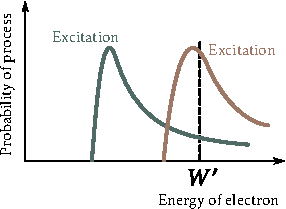
\includegraphics[scale=1]{figures/ch_12/fig_12_6.pdf}
		\caption[]{}
		\label{fig:12_6}
	\end{center}
	\vspace{-0.8cm}
\end{figure}

\textbf{Ion hóa bởi ánh sáng}. Bức xạ điện từ được lượng tử hóa dưới dạng hạt cơ bản được gọi là \textbf{photon}.
Năng lượng của một photon bằng $\hslash\omega$, với $\hslash$ là hằng số Plank chia cho $2\phi$ [xem \eqn{7_43}], và $\omega$ là tần số góc của bức xạ.
Một photon có thể được hấp thụ bởi một phân tử, và năng lượng của nó có thể dùng để kích thích hoặc ion hóa phân tử này.
Trong trường họp này, sự ion hóa của một phân tử được gọi là \textbf{sự quang ion hóa}.
Bức xạ cực tím có khả năng quang ion hóa trực tiếp.
Năng lượng của một photon ánh sáng khả vi không đủ để tách một electron khỏi phân tử.
Do đó, bức xạ khả vi không có khả năng quang ion hóa.
Nhưng nó có thể là nguyên nhân bởi vì \textbf{quang ion hóa từng phần}.
Quá trình này diễn ra trong hai bước.
Trong bước đầu tiên, một photon đưa phân tử vào 
trạng thái kích thích.
Ở bước thứ hai, phân tử kích thích bị ion hóa bởi vì sự va chạm với một phân tử khác.

Các bức xạ ngắn xuất hiện trong sự phóng điện trong chất khí có khả năng quang ion hóa trực tiếp.
Một electron di chuyển đủ nhanh không chỉ ion hóa một phân tử khi va chạm mà còn có thể đưa ion đến trạng thái kích thích.
Sự chuyển dời ion về trạng thái nền đi kèm với bức xạ có tần số cao hơn của một phân tử trung hòa.
Năng lượng của một photon trong bức xạ này có khả năng quang ion hóa trực tiếp.

\textbf{Phát xạ electron trên bề mặt điện cực.} Các electron có thể được truyền đến không gian xảy ra sự phóng điện do sự phát xạ của chúng trên bề mặt các điện cực.
Các loại phát xạ như phát xạ nhiệt (electron nhiệt), electron thứ cấp và tự phát xạ electron đóng vai trò chủ yếu trong nhiều dạng phóng điện.

\textbf{Phát xạ nhiệt} là tên gọi của sự phát xạ electron bởi các chất rắn hoặc chất lỏng được nung nóng.
Do các electron tự do trong kim loại có vận tốc khác nhau theo định luật phân bố, luôn tồn tại những electron mà năng lượng đủ để vượt qua rào thế và rời khỏi khối kim loại.
Số lượng electron như vậy tại nhiệt độ phòng là rất nhỏ.
Mặc dù vậy, khi tăng nhiệt độ, số electron có khả năng rời kim loại tăng rất nhanh và tương đối lớn tại nhiệt độ trên cỡ \SI{1000}{\kelvin}.

Sự \textbf{phát xạ electron thứ cấp} là sự phát xạ electron từ bề mặt của một chất lỏng hoặc chất rắn khi bị bắn phá bởi các electron hoặc ion.
Tỉ lệ giữa số lượng electron phát ra (thứ cấp) và số lượng hạt sinh ra sự phát xạ được gọi là hệ số phát xạ electron thứ cấp.
Khi dùng electron để bắn vào bề mặt một tấm kim loại, giá trị hệ số này có thể thay đổi từ $0.5$ (cho beri) cho tới $1.8$ (cho bạch kim).

\textbf{Tự phát xạ electron} (hoặc \textbf{phát xạ lạnh}) là sự phát xạ electron từ bề mặt một kim loại khi điện trường rất lớn ($\sim\SI{e8}{\volt\per\metre}$) được thiết lập gần bề mặt.
Hiệu ứng này còn được gọi là phát xạ electron cảm ứng trường.

\section{Phóng điện Plasma}\label{sec:12_5}

Các dạng phóng điện tự duy trì được thể hiện bởi mức độ ion hóa rất cao.
Một chất khí được ion hóa mạnh, với tổng điện tích của các electron và ion trong từng đơn vị thể tích 
bằng (hoặc gần bằng) không, được gọi là \textbf{plasma}.
Plasma là một trạng thái đặc biệt của vật chất.
Vật chất trong lõi Mặt trời và các ngôi sao khác có nhiệt độ hàng triệu Kelvin đều ở trạng thái này.
Một chất plasma sinh ra do nhiệt độ cao của chất đó được gọi là \textbf{plasma nhiệt độ cao} (hoặc \textbf{plasma đẳng nhiệt}).
Một chất plasma \textbf{phóng điện}, như tên gọi của nó, là chất được sinh ra trong sự phóng điện trong chất khí.

Để một chất plasma trong trạng thái bền, cần có các quá trình diễn ra bù đắp các ion giảm dần do sự tái hợp.
Trong các plasma năng lượng cao, điều này đạt được bởi sự nhiệt ion hóa, trong plasma phóng điện, do sự ion hóa va chạm bởi các electron gia tốc bởi một điện trường.
Tầng điện li (một trong những lớp của bầu khí quyển) là một biến thể đặc biệt của plasma.
Mức độ ion hóa cao của các phân tử ($\sim 1\%$) được duy trì ở tầng điện ly do sự quang ion hóa do bức xạ sóng ngắn của Mặt trời.

Các electron trong một plasma phóng điện tham gia vào hai chuyển động---hỗn loạn với vận tốc trung bình $\average{v}$ và một chuyển động có trật tự hướng ngược lại với $\vec{E}$ với vận tốc trung bình $\average{u}$ nhỏ hơn nhiều so với $\average{v}$.

\begin{figure}[t]
	\begin{center}
		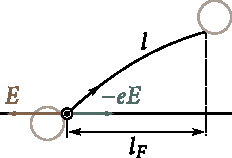
\includegraphics[scale=1]{figures/ch_12/fig_12_7.pdf}
		\caption[]{}
		\label{fig:12_7}
	\end{center}
	\vspace{-0.8cm}
\end{figure}

Chúng ta sẽ chứng minh rằng điện trường không chỉ dẫn tới chuyển động có trật tự của electron trong plasma mà còn tăng vận tốc $\average{v}$ của chuyển động hỗn loạn.
Giả sử rằng tại thời điểm điện trường được bật lên, chất khí chứa một lượng nhất định electron với vận tốc trung bình tương ứng với nhiệt độ $\ab{T}{g} (m\average{v}^2/2 = 3k\ab{T}{g}/2$.
Trong khoảng thời gian giữa hai va chạm liên tiếp với các phân tử, một electron đi được đoạn đường trung bình $l$ (\fig{12_7}; quỹ đạo của electron bị cong đi một chút dưới tác động của lực $-eE$).
Công thực hiện lên electron bởi trường là
\begin{equation}\label{eq:12_16}
    A = e E l_F,
\end{equation}

\noindent
với $l_F$ là thành phần chiếu của quỹ đạo electron trên phương của lực tác động lên nó
Do va chạm với các phân tử, hướng chuyển động của electrong liên tục thay đổi một cách hỗn loạn.
Do vậy, độ lớn và dấu của $l$ cũng thay đổi theo.
Đây là lý do công trong \eqn{12_16} với các phần khác nhau của quỹ đạo thay đổi về cả chiều về độ lớn.
Ở một số đoạn, trường tăng năng lượng của electron, trong khi giảm ở những đoạn khác.
Nếu không có chuyển động có trật tự, giá trị trung bình của $l$, và theo đó là công trong \eqn{12_16} sẽ bằng không.
Khi có chuyển động trật tự, giá trị trung bình của công $A$ khác không, nó bằng
\begin{equation}\label{eq:12_17}
    \average{A} = e E \average{u} \tau = e E \average{u} \frac{l}{\average{v}},
\end{equation}

\noindent
với $\tau$ là thời gian trung bình cần có để electron đi hết quãng đường tự do ($\average{u} \ll \average{v}$)

Do đó, điện trường, tính trên trung bình, tăng năng lượng của electron
Một mặt, một electron khi va chạm với một phân tử chuyển đi một phần năng lượng của mình.
Nhưng như chúng ta đã thấy ở phần trước, phần $\delta$ của năng lượng chuyển đến một va chạm đàn hồi là rất nhỏ---nó\footnote{Theo \eqn{12_12} trong một va chạm trực diện $\delta = 4(m/M)$. Khi electron và phân tử chỉ va quệt nhẹ, ta có $\delta\approx 0$.} có giá trị trung bình $\delta = 2(m/M)$ (với $m$ là khối lượng một electron, và $M$ là của một phân tử). 

Trong một khí hiếm (với $l$ lớn hơn) và với cường độ trường $E$ đủ lớn, công $\average{A}$ [\eqn{12_17}] có thể chạm ngưỡng năng lượng trung bình $m\average{v^2}\average{\delta}/2$ chuyển cho một tử trong mỗi va chạm.
Kết quả là sự tăng vọt trong năng lượng chuyển động hỗn loạn của các electron.
Giá trị này cuối cùng sẽ đạt đủ để kích thích hoặc ion hóa một phân tử.
Kể từ khi này, một số va chạm sẽ không còn đàn hồi và đi kèm với một sự mất năng lượng lớn
Do đó, tỉ lệ trung bình $\average{\delta}$ của năng lượng truyền đi tăng lên.

Khi này, các electron đạt đủ năng lượng cần để ion hóa không phải trong một khoảng giữa va chạm, mà tăng dần qua nhiều lần va chạm.
Sự ion hóa này dẫn đến sự xuất hiện một lượng lớn các electron và ion dương---một plasma được sinh ra.

Năng lượng của electron trong plasma được xác định bởi điều kiện giá trị công trung bình thực hiện bởi điện trường lên một điện tường trong một khoảng giữa hai va chạm bằng năng lượng trung bình chuyển từ electron khi va chạm với một phân tử
\begin{equation*}
    e E \average{u} \frac{1}{\average{v}} = \frac{m \average{v^2}}{2} \average{\delta}.
\end{equation*}

\noindent
Ở đây, $\delta$ là một hàm phức tạp của $\average{v}$.

Thí nghiệm cho thấy rằng các electron trong chất plasma phóng điện tuân theo phân bố vận tốc Maxwell.
Do tương tác rất yếu giữa các electron với phân tử (trong một va chạm đàn hồi $\delta$ là rất nhỏ, trong khi số lượng tương đối của các va chạm không đàn hồi là không đáng kể), tốc độ trung bình của chuyển động hỗn loạn của electron lớn hơn nhiều tốc độ ứng với nhiệt độ $\ab{T}{g}$ của chất khí.
Nếu chúng ta đặt nhiệt độ của electron $\ab{T}{e}$ xác định từ phương trình $m\average{v^2} = 3k\ab{T}{e}/2$, ta có được một giá trị trên khoảng vài chục ngàn kelvin.
Việc hai nhiệt độ $\ab{T}{g}$ và $\ab{T}{e}$ không thể trùng nhau cho thấy rằng không tồn tại cân bằng nhiệt động giữa electron và các phân tử trong một chất plasma phóng điện\footnote{Năng lượng trung bình của các phân tử, electron và ion trong một chất plasma nhiệt độ cao là bằng nhau. Điều này giải thích tên gọi khách của nó---plasma đoạn nhiệt.}
Mật độ hạt tải dòng trong plasma là rất cao.
Do đó, plasma là một chất dẫn điện rất tốt.
Độ linh hoạt của electron lớn hơn của ion khoảng 3 cỡ độ lớn.
Cho nên dòng trong plasma chủ yếu được thiết lập bởi các electron

\section{Glow Discharge}\label{sec:12_6}

Một sự phóng điện huỳnh quang diễn ra tại áp suất thấp.
Ta có thể quan sát hiện tượng này trong một ống thủy tinh dài khoảng \SI{0.5}{\metre} với các điện cực kim loại phẳng hàn vào hai đầu (\fig{12_8}).
Điện áp khoảng $\sim\SI{1000}{\volt}$ được đặt vào các điện cực.
Trong ống sẽ không có dòng tại áp suất khí quyển.
Nếu áp suất được hạ xuống, ở khoảng \SI{50}{\mmHg} một sự phóng điện diễn ra dưới dạng một dây mảnh phát sáng nối giữa anode và cathode.
Sự giảm áp suất đi kèm với sự dày lên của dây này, và tại khoảng \SI{5}{\mmHg} tiết diện của sự phóng điện trải dài toàn bộ ống---diễn ra sự phóng điện huỳnh quang.
Cấu tạo cơ bản được biểu diễn ở \fig{12_8}
Gần cathode là một tấm mỏng phát quang được gọi là \textbf{tấm phát quang cathode}.
Giữa cathode và tấm phát quang là \textbf{vùng tối Aston}.
Tại phía bên kia của tấm phát quang là một tấm phát quang yếu hơn, trông có vẻ tối và được gọi là \textbf{vùng tối} \textbf{cathode} (hoặc \textbf{Crookes})
Tấm này đặt tại biên một vùng sáng gọi là \textbf{quầng sáng âm}.
Tất cả những tấm trên hình thành phần cathode của ống huỳnh quang.

\begin{figure}[t]
	\begin{center}
		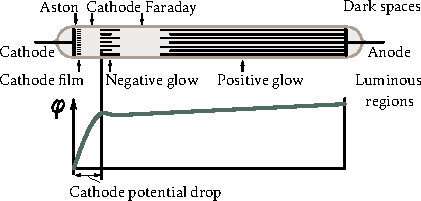
\includegraphics[scale=1]{figures/ch_12/fig_12_8.pdf}
		\caption[]{}
		\label{fig:12_8}
	\end{center}
	\vspace{-0.8cm}
\end{figure}

Quầng sáng âm được nối tiếp bởi \textbf{vùng tối Faraday}.
Không có ranh giới rõ ràng giữa hai vùng này.
Phần còn lại của ống chứa đầy một chất khí phát quang; nó được gọi là \textbf{cột dương}.
Tại áp suất thấp, phần cathode của ống huỳnh quang và vùng tối Faraday trở nên rộng hơn, trong khi cột dương trở nên ngắn hơn.
Tại áp suất trên khoảng \SI{1}{\mmHg}, cột dương tách ra thành nhiều lớp sáng tối xen kẽ-\textbf{strata}.

Sự đo đạc với hỗ trợ của các đầu dò (các đoạn dây mỏng hàn vào các điểm khác nhau dọc theo ống) và cac phương thức khác cho thấy điện thế nay đổi không đều dọc theo ổng (tham khảo đồ thị \fig{12_8}).
Gần như toàn bộ độ sụt thế rơi vào ba phần đầu tiên của ống phòng cho đến vùng tối cathode.
Phần điện thế đặt lên ống này được gọi là \textbf{độ sụt thế cathode}.

The main processes needed to maintain a glow discharge occur in its cathode part.
The other parts of the discharge are not significant, they may even be absent (with a small spacing of the electrodes or at a low pressure).
There are two main processes---secondary electron emission from the cathode produced by its bombardment with positive ions, and collision ionization of the gas molecules by electrons.

The positive ions accelerated by the cathode potential drop bombard the cathode and knock electrons out of it.
These electrons are accelerated by the electric field in the Aston dark space.
Acquiring sufficient energy, they begin to excite the gas molecules, owing to which the cathode luminous film appears.
The electrons that fly without any collisions into the region of the cathode dark space have a high energy, and as a result they ionize the molecules more frequently than they excite them (see the graphs in \fig{12_6}).
Thus, the intensity of glowing of the gas diminishes, but in return many electrons and positive ions appear.
The ions produced first have a very low velocity.
As a result, a positive space charge is formed in the cathode dark space.
This leads to redistribution of the potential along the tube and to the appearance of the cathode potential drop.

The electrons appearing in the cathode dark space penetrate into the negative glow region that is characterized by a high concentration of electrons and positive ions and by a total space charge close
to zero (a plasma).
Therefore, the field strength here is very low.
Owing to the high concentration of electrons and ions, an intensive recombination process goes on in the negative glow region.
It is attended by the emission of the energy liberated during this process. Thus,
the negative glow is mainly a glow of recombination.

The electrons and ions penetrate from the negative glow region into the Faraday dark space because of diffusion (there is no field on the boundary between these regions, but in return there is a high gradient of electron and ion concentration).
The lower concentration of the charged particles greatly diminishes the probability of recombination in the Faraday dark space.
This is why the latter space seems to be dark.

A field is already present in the Faraday dark space.
The electrons carried away by this field gradually accumulate energy so that the conditions needed for the existence of a plasma finally appear.
The positive column is a gas-discharge plasma.
It plays the part of a conductor joining the anode to the cathode parts of the discharge.
The glow of the positive column is mainly due to transitions of excited molecules to their ground state.
Molecules of different gases emit radiation of different wavelengths in such transitions.
Therefore, the glow of the positive column has a characteristic colour for each gas.
This circumstance is taken advantage of in glow tubes for manufacturing luminous inscriptions and advertisements.
These inscriptions are the positive column of a glow discharge.
Neon gas-discharge tubes produce a red glow, argon ones a bluish-green glow, etc.

If the electrode spacing is gradually diminished, the cathode part of the discharge remains unchanged whereas the length of the positive column diminishes until this column disappears completely.
Next, the Faraday dark space disappears, and the length of the negative glow begins to decrease, the position of the boundary of this glow with the cathode dark space remaining unchanged.
When the distance from the anode to this boundary becomes very small, the discharge stops.

If the pressure is gradually lowered, the cathode part of the discharge extends over a greater and greater part of the interelectrode space, and finally the cathode dark space extends over almost the entire tube.
The glow of the gas in this case stops being noticeable but in return the tube walls begin to glow with a greenish colour.
The majority of the electrons knocked out of the cathode and accelerated by the cathode potential drop reach the tube walls without colliding with molecules of the gas and cause the walls to glow upon
striking them.
For historical reasons, the stream of electrons emitted by the cathode of a gas-discharge tube at very low pressures was called \textbf{cathode rays}.
The glow produced by bombardment with fast electrons
is called \textbf{cathodoluminescence}.

If a narrow canal is made in the cathode of a gas-discharge tube, part of the positive ions penetrate into the space beyond the cathode and form a sharply bounded beam of ions called canal (or positive) rays.
Beams of positive ions were first obtained in exactly this way.

\section{Arc Discharge}\label{sec:12_7}

In 1802, the Russian physicist Vasili Petrov (1761-1834) discovered that when contacting carbon electrodes connected to a large galvanic battery are moved apart, a concentrated light flares up between
the electrodes.
When the electrodes are horizontal, the heated luminescent gas bends in the shape of an arc.
This is why the phenomenon discovered by Petrov was called an \textbf{electric arc}.
The current in the arc may reach enormous values (from \SIrange{e3}{e4}{\ampere}) at a voltage
of several scores of volts.

An arc discharge can proceed at both a low (of the order of several millimetres of mercury) and a high (up to $1000$ atmospheres) pressure.
The main processes maintaining the discharge are thermionic emission from the heated cathode surface and thermal ionization of the molecules due to the high temperature of the gas in the space between the electrodes.
Almost the entire interelectrode space is filled with a high-temperature plasma.
It is the conductor through which the electrons emitted by the cathode reach the anode.
The temperature of the plasma is about \SI{6000}{\kelvin}.
In a superhigh-pressure arc, the temperature of the plasma may reach \SI{10000}{\kelvin} (we remind our reader that the temperature of the Sun's surface is \SI{5800}{\kelvin}).
Owing to bombardment by positive ions, the cathode is heated to about \SI{3500}{\kelvin}.
The anode, bombarded by a powerful stream of electrons, is heated still more.
As a result, the anode intensively evaporates, and a depression---a crater---is formed on its surface.
The crater is the brightest place in an arc.

An arc discharge has a dropping volt-ampere characteristic (\fig{12_9}).
The explanation is that a current increase is attended by a growth in the thermionic emission from the cathode and in the degree of ionization of the gas-discharge space.
As a result, the resistance of this space diminishes at a greater rate than that of the current increase.

\begin{figure}[t]
	\begin{center}
		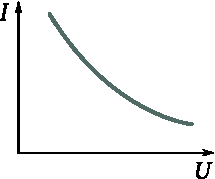
\includegraphics[scale=1]{figures/ch_12/fig_12_9.pdf}
		\caption[]{}
		\label{fig:12_9}
	\end{center}
	\vspace{-0.8cm}
\end{figure}

Apart from the thermionic arc described above (\ie, a discharge due to thermionic emission from the heated surface of the cathode) an \textbf{arc with a cold cathode} is also encountered.
Usually liquid mercury poured into a cylinder from which the air has been evacuated is the cathode of such an arc.
The discharge occurs in the mercury vapour.
The electrons fly out of the cathode as a result of autoelectronic emission.
The strong field at the cathode surface needed for this to occur is set up by the positive space charge formed by the ions.
The electrons are emitted not by the entire surface of the cathode, but by a small luminous and continuously moving cathode spot.
The temperature of the gas in this case is not high.
The molecules in the plasma are ionized, as in a glow discharge, as a result of collisions with the electrons.

\section{Spark and Corona Discharges}\label{sec:12_8}

A spark discharge is produced when the electric field strength reaches the breakdown value $\ab{E}{br}$ for the given gas.
The value of $\ab{E}{br}$ depends on the gas pressure; it is about \SI{3}{\mega\volt\per\metre}  (\SI{30}{\kilo\volt\per\centi\metre}) for air.
The value of $\ab{E}{br}$ varies with the pressure.
According to the experimentally established \textbf{Paschen law}, the ratio of the breakdown field strength to the pressure is approximately constant:
\begin{equation*}
    \frac{\ab{E}{br}}{p} \approx \text{constant}.
\end{equation*}

A spark discharge is attended by the formation of a brightly luminous tortuous branched canal along which a short-time strong current pulse flows.
An example is lightning; its length may be up to \SI{10}{\kilo\metre}, the diameter of the canal up to \SI{40}{\centi\metre}, the current may reach $100 000$ and more amperes, and the duration of the pulse is about \SI{e-4}{\second}.
Every stroke of lightning consists of several (up to $50$) pulses flowing along the same canal; their total duration (together with the intervals between the pulses) may reach several seconds.
The temperature of the gas in the spark canal is up to \SI{10000}{\kelvin}.
The rapid strong heating of the gas leads to a sharp growth in the pressure and the production of shock and sound waves.
This is why a spark discharge is attended by sound phenomena---from a weak crackling for a low-power spark to peals of thunder accompanying a stroke of lightning.

The appearance of a spark is preceded by the formation in the gas of a greatly ionized canal known as a streamer.
The latter is obtained by overlapping of the separate electron avalanches appearing along the path of the spark.
The forefather of each avalanche is an electron released by photoionization.
How a streamer develops is shown in \fig{12_10}.
Assume that the field strength has a value such that an electron flying out of the cathode as a result of some process or other acquires an energy sufficient for ionization along its free path.
This causes multiplication of the electrons to occur---an avalanche is formed (the positive ions appearing during this process do not play a noticeable part owing to their much smaller mobility; they only set up the space charge resulting in redistribution of the potential).
The short-wave radiation emitted by an atom that lost one of its inner electrons when ionized (this radiation is shown by wavy lines in the figure) produces photoionization of the molecules, the detached electrons giving birth to more and more new avalanches.
After overlapping of the avalanches, a well-conducting canal---a streamer---is formed along which a powerful stream of electrons flows from the cathode to the anode---breakdown occurs.

\begin{figure}[t]
	\begin{center}
		
\includegraphics[scale=1]{figures/ch_12/fig_12_10.pdf}
		\caption[]{}
		\label{fig:12_10}
	\end{center}
	\vspace{-0.8cm}
\end{figure}

If the electrodes have a shape at which the field in the space between them is approximately homogeneous (for example, they are spheres of a sufficiently great diameter), then breakdown occurs at a quite definite voltage $\ab{U}{br}$ whose value depends on the distance between the spheres $l$ ($\ab{U}{br} = \ab{E}{br}l$).
This underlies the design of a spark voltmeter used to measure high voltages (from \SIrange{e3}{e5}{\volt}).
During such measurements, the maximum distance $\ab{l}{max}$ is determined at which a spark appears.
Next multiplying $\ab{E}{br}$ by $\ab{l}{max}$, we get the value of the voltage being measured.

If one of the electrodes (or both) has a very great curvature (for example, the electrode is a thin wire or a sharp point), then when the voltage is not too high, a so-called \textbf{corona discharge} is produced.
When the voltage grows, this discharge transforms into a spark or an arc discharge.

In a corona discharge, the ionization and excitation of the molecules occur not in the entire interelectrode space, but only near an electrode having a small radius of curvature, where the field strength reaches values equal to or greater than $\ab{E}{br}$.
The gas glows in this part of the discharge.
The glow has the form of a corona surrounding the electrode, and this explains the name given to this kind of discharge.
A corona discharge from a point has the form of a luminous brush, and for this reason it is sometimes known as a \textbf{brush discharge}.
Positive and negative coronas are distinguished depending on the sign of the corona electrode.
The \textbf{external corona} region is between the corona layer and the non-corona electrode.
Breakdown conditions ($E\gg\ab{E}{br}$) exist only within the limits of the corona layer.
We can, therefore, say that a corona discharge is incomplete breakdown of the gas space.

With a negative corona, the phenomena at the cathode are similar to those at the cathode of a glow discharge.
The positive ions accelerated by the field knock electrons out of the cathode.
These electrons produce ionization and excitation of the molecules in the corona layer.
In the external region of the corona, the field is not sufficient to impart the energy needed for ionization or excitation of the molecules to the electrons.
For this reason, the electrons that penetrate into this region drift toward the anode under the action of the field.
Part of the electrons are captured by the molecules, the result being the formation of negative ions.
Thus, the current in the external region is due only to negative carriers-electrons and negative ions.
The discharge in this region is of a semi-self-sustained nature.

In a positive corona, the electron avalanches are conceived at the outer boundary of the corona and fly toward the corona electrodethe anode.
The appearance of electrons giving birth to avalanches is due to photoionization produced by the radiation of the corona layer.
The current carriers in the external region of the corona are the positive ions that drift to the cathode under the action of the field.

If both electrodes have a great curvature (two corona electrodes), processes occur near each of them that are characteristic of a corona electrode of the given sign.
Both corona layers are separated by an external region in which opposite streams of positive and negative current carriers travel.
Such a corona is called a bipolar one.

The self-sustained gas discharge mentioned in \sect{12_5} when treating counters is a corona discharge.

The thickness of the corona layer and the discharge current grow with an increasing voltage.
At a low voltage, the size of the corona is small, and its glow is hard to notice.
Such a microscopic corona is produced near a sharp point off which an electric wind flows (see
\sect{3_1}).

The bluish electrical glow caused by corona discharge on masts and other high parts of a ship at sea before and after electrical storms was called St. Elmo's fire in olden days.

In high-voltage facilities, for example, in high-tension transmission lines, a corona discharge leads to the harmful leakage of current.
Measures therefore have to be taken to prevent it.
For this purpose, for instance, the wires of high-tension lines are taken of a sufficiently large diameter, which is the greater, the higher is the voltage of the line.

The corona discharge has found a useful application in engineering in electrical filters.
The gas being purified flows through a tube along whose axis a negative corona electrode is arranged.
The negative ions present in a great number in the external region of the corona settle on the particles or droplets polluting the gas and are carried along with them to the external non-corona electrode.
Upon reaching the latter, the particles become neutralized and settle on it.
Later, blows are struck at the tube and the sediment formed by the precipitated particles drops into a collector.
